\documentclass[12pt]{article}

\usepackage{../thesis}

\usepackage{tikz} 

\begin{document}

\pagestyle{empty}

\begin{tikzpicture}
    \node[anchor=south west,inner sep=0] (image) at (0,0) {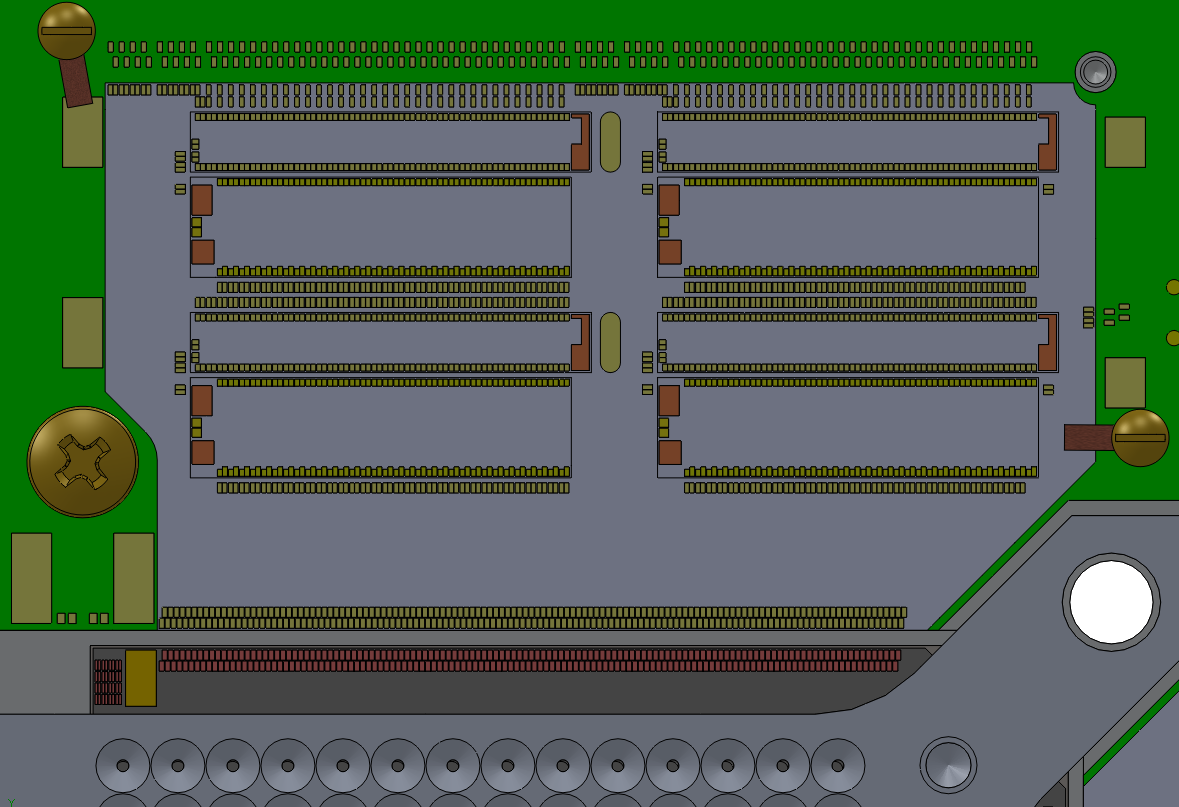
\includegraphics[height=3.0in]{../images/ch5-wiring-chip-schematic.png}};
    \begin{scope}[x={(image.south east)},y={(image.north west)}]
	    % \draw[help lines,xstep=.1,ystep=.1] (0,0) grid (1.0,1);
		% \foreach \x in {0,1,...,9} { \node [anchor=north] at (\x/10,0) {0.\x}; }
		% \foreach \y in {0,1,...,9} { \node [anchor=east] at (0,\y/10) {0.\y}; }
		
        \node at (0.35,0.82) {\textbf{MUX11C}}; 
        \node at (0.75,0.82) {\textbf{MUX11C}}; 
        \node at (0.35,0.575) {\textbf{MUX11C}}; 
        \node at (0.75,0.575) {\textbf{MUX11C}}; 
        
        \node at (0.35,0.72) {\textbf{interface}}; 
        \node at (0.75,0.72) {\textbf{interface}}; 
        \node at (0.35,0.475) {\textbf{interface}}; 
        \node at (0.75,0.475) {\textbf{interface}}; 

        \node at (0.35,0.32) {\textbf{Wiring Chip}}; 

        \node at (0.35,0.145) {\textbf{Detector Wafer}}; 

       \draw[black,ultra thick,<->] (.5,0.35) -- (0.84,0.35) node[midway,below] {\SI{2}{\cm}}; % scale bar --- interace chip is 0.323 picture units long, 19 mm
    \end{scope}
\end{tikzpicture}

\end{document}
